%!TEX root = tesi.tex




\begin{comment}
~ "Classically, and to all orders of perturbation theory, the 
\section{Electric-magnetic duality in three and four dimensions}


electric and magnetic
   theories have different moduli spaces of vacua – it is only after taking nonperturbative
   effects into account that they are seen to be identical. For example, in
   the electric theory there is a classical constraint rankhMi ≤ Nc. In the dual theory,
   M is an independent field whose expectation value is unconstrained to all orders of
   perturbation theory – the constraint arises in the dual theory by quantum effects!"

   pag 27 di lectures

\end{comment}

\section{Electric-magnetic duality in three and four dimensions}


\begin{comment}
\subsubsection{Moduli space of $4D \; \mN=1$ SQCD with $SU(N_c)$ gauge group and $N_f$ flavors}
As a concrete example of moduli space we will analyse $SU(N_c)$ SQCD with $N_f$ flavors.
Its classical lagrangian contains no superpotential and is given by two terms, generating \emph{D-terms} equations
\begin{equation}
\mathcal{L } =  \mathcal{L }_{SYM} + \mathcal{L }_{matter} 
\end{equation}
we refer to appendix \ref{appendice_susy} for their explicit form.

The global non anomalous symmetry group of the theory is $SU(N_f)_L \times SU(N_f)_R \times U(1)_B \times U(1)_R$. 
The matter content of the theory consists of $N_f$ $(Q_i, \tilde{Q}^{\tilde{j}})$ pairs of chiral fields, charged under \emph{left}  \emph{right} flavor symmetries respectively. 

\end{comment}
\begin{lstlisting}
-------- Roba da dire nel capitolo ---------
 ~Phases of gauge theories?(asympt. free, non abelian coulomb/magnetic..)
 ~Region where duality is correct because of unitary?
 ~Use of superconformal algebra
 ~Anomaly free global symmetries
 ~Different gauge group: scale invariant theory
  ~Construct the dual from gauge invariant operators: they make sense and are consistent with other symmetries & anomalies
 ~Superpotential allowed by charges
 ~'t'Hooft anomalies
 ~Different group con be used
	\end{lstlisting}


\section{Four dimensional dualities}

We will start our analysis on eletric-magnetic duality studying the first pair of theories that were discovered to be dual in \cite{Seiberg:1994pq}.  
We are gonna analyse the properties of these theory in order to better understand the features of the duality.

\subsection*{Seiberg Duality --- $SUN(N)$ SQCD with $N_f$ flavors}
The electric theory is a $SU(N_c) $ supersymmetric gauge theory with $N_f$ flavours.
Its non anomalous global symmetry group is $SU(N_f)_L \times SU(N_f)_R \times U(1)_B \times U(1)_R $. 

The classical lagrangian doesn't have a superpotential and in terms of superfield is written as
\begin{equation}
 \mathcal{L} = \int d^2 \theta \; Tr ( W_{\alpha} W^{\alpha} ) + 
 \int d^2 \theta \, d^2 \bar{\theta} \;  {Q}^{\dagger} e^{ V} Q +
 \int d^2 \theta \, d^2 \bar{\theta} \; {\tilde{Q}^{\dagger}} e^{- V} \tilde{Q}
 \end{equation} 
$Q$ and $\tilde{Q}$ represent left and right quark superfield respectively.\\
The charges of the fields are summarized in the table below.
\begin{table}[h!]
 \begin{tabular}{c | c |  c c c c }
 & $SU(N_c) $& $SU(N_f)_L$  &$SU(N_f)_R $  & $U(1)_B$ &  $U(1)_R$ \\
\hline
$Q$ & $N_c$ & $N_F$ & $1$   &  $1$  & $ \frac{N_f - N_c}{N_f}$  \\
$\tilde{Q}$ &$\overline{N_c} $ &  $1$ & $\overline{ N_F}$   & $-1$   &  $\frac{N_f - N_c}{N_f}$   \\	 
 \end{tabular}
	\centering
 \caption{Charges of the electric theory}
\end{table}
Mixing the R-symmetry with the baryon symmetry we can set the quark R-charges to be equal.
Moreover, the value of the R-charge is fixed by the triangle anomaly $SU(N_c)^2 \, U(1)_R $, given by diagrams with two exiting gluons and R-symmetry current inserted in the cross 
\begin{center}
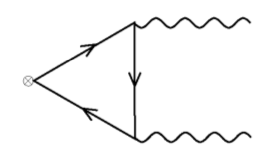
\includegraphics[scale=0.6]{r-symm_anomlay.png}
\end{center}
Every fermion in the theory contributes to the anomaly which, as a result, is proportional to the R-charge of the fermion running in the loop and the Dynkin index of its representation
\begin{align*}
R_{gaugino} T (\hbox{Ad}) + \sum_{ f} (& R_{f} - 1)  T(r)   = 0 \\
N_c + \frac{1}{2}\,  2 N_f (R_Q -1)  = 0 \quad & \rightarrow \quad R_Q = \frac{N_f - N_c}{N_f}
\end{align*}
where we set  the gaugino R-charge to $1$ in order to have gluons without charge.\\


\subsubsection{Classical moduli space}
Since there is no superpotential, the classical moduli space of the theory is given by \emph{D-terms} only. 
They can be read from the on-shell lagrangian and are given by
\begin{equation}
 D^a = g \left( Q^{*i} T^a Q_i - \tilde{Q}^{* i} T^a \tilde{Q}_i \right) = 0
\end{equation}
where $T^a$ are the gauge group generators in fundamental or antifundamental representation, color indices are suppressed and $i$ is a flavour index.

After considering gauge and global symmetries, the squark \emph{VEVs}, represented as $N_f \times N_c$ matrices, that satisfy the D-term equation are
\begin{equation}
Q = \tilde{Q} = 
\begin{pmatrix}
 a_1 & 		&	 &	 & \vdots \\
	 & a_2  & 	 & 	 & \vdots \\  	
 	 & 		&	\ddots &	 &\vdots  \\
	 &  & 	 & 	a_{N_f}  & \vdots
\end{pmatrix} 
 \\
\end{equation}
for  $N_f \le N_c$ and $a_i$ generic and
\begin{equation}
Q  = 
\begin{pmatrix} 
	 a_1 & 		&	 &	  \\
	 & a_2  & 	 & 	 \\  	
 	 & 		&	\ddots &	   \\
	 &  & 	 & 	a_{N_c}  \\
	 \dots & \dots & \dots & \dots\\ 
\end{pmatrix} 
\quad
\tilde{Q} = 
\begin{pmatrix}
 \tilde{a}_1 & 		&	 &	  \\
	 & \tilde{a}_2  & 	 & 	 \\  	
 	 & 		&	\ddots &	   \\
	 &  & 	 & 	\tilde{a}_{N_c}  \\
	 \dots & \dots & \dots & \dots\\ 
\end{pmatrix} 
\end{equation}
for $N_f \geq N_c$ and $ | a_i|^2 - | \tilde{a}_i |^2 = a $ indepdent of $i$.

We can try to understand why for different number of flavors the theory has qualitatively different moduli spaces. 
As we said in the previous section, we can solve the D-term equation by finding holomorphic gauge invariant polynomial in the operators and modding out classical relations between them.
For $N_f \le N_c$ we can only construct \emph{mesons} out of squarks
\begin{equation}
  M^i_j = Q^i \tilde{Q}_j
 \end{equation} 
where color indices are summed. 
Mesons have maximal rank since $N_f \le N_c$ and there are no  classical to impose on them. 
They can be diagonalized in the same way we put the squarks \emph{VEVs} in diagonal form.\\ 
When $N_f \geq N_c$ the mesons cannot have maximal rank anymore, it can be at most $N_c$.
There are additional gauge invariant operators that can be constructed: \emph{baryons}, that are defined as
\begin{align}
 B_{ i_1, \dotsc, i_{N_f - N_c}} = \epsilon_{i_1, \dotsc, i_{N_f - N_c}, j_1 ,\dotsc, j_{N_c}} \epsilon^{a_1 , \dotsc, a_{N_c}} Q^{j_1}_{a_1} \dots Q^{j_{N_c}}_{a_{N_c}}
 \\
 \tilde{B}_{ i_1, \dotsc, i_{N_f - N_c}} = \epsilon^{i_1, \dotsc, i_{N_f - N_c}, j_1 , \dotsc, j_{N_c}} \epsilon_{a_1 , \dotsc, a_{N_c}} \tilde{Q}_{j_1}^{a_1} \dots \tilde{Q}_{j_{N_c}}^{a_{N_c}}
\end{align}
Mesons and baryons can be written down explicitly (ignoring null components for baryons)
\begin{align}
M =& \begin{pmatrix}
a_1 \tilde{a_1} & & & & & \\
				& a_2 \tilde{a_2}	& 		&		 & & \\
				&				 	& \ddots&		& 	& \\
				&					&		& a_{N_c} \tilde{a_{N_c}} & \\
				& & & & & \\	
\end{pmatrix}
\\
B_{1 2 \dots {N_c}} =& a_1 a_2 \dots a_{N_c} 
\\
\tilde{B}_{1 2 \dots {N_c}} =& \tilde{a_1} \tilde{a_2}\dots \tilde{a_{N_c}}
\end{align}
We can see that if the meson has rank less than $N_c$, then $B$ or $\tilde{B}$ (or both) has to vanish and the other has rank one. If the meson rank is $N_c$ both $B$ and $\tilde{B}$ have rank one.

Moreover that are classical constraints between mesons and baryons, but depend on the number of flavor.
For example for $N_f = N_c$ we have $ det \,( M) - B \tilde{B} = 0$




















\newpage
\begin{comment}
The magnetic theory is a theory with the same global symmetries as the electric theory, but the gauge group is now $SU(N_f - N_c)$ and in addition there are $N_f^2$ fields, that we will call mesons. 
Dual quarks will be represented as $q,\tilde{q}$ and mesons as $M^i_{\tilde{j}} $
The charges for the magnetic theory are given by


\begin{table}[h!]
 \begin{tabular}{c | c |  c c c c }
 & $SU(N_c) $& $SU(N_f)_L$  &$SU(N_f)_R $  & $U(1)_B$ &  $U(1)_R$ \\
\hline
$q$ & $N_c$ & $N_F$ & $1$   &  $ \frac{N_c}{N-f-N_c} $  & $ \frac{N_c}{N_f}$  \\
$\tilde{q}$ &$\overline{N_c} $ &  $1$ & $\overline{ N_F}$   & $- \frac{N_c}{N-f-N_c}$   &  $ \frac{N_c}{N_f}$   \\	 
$M^i_{\tilde{j}} $ & $1$ & $N_f$ & $\overline{N_f} $ & $0$ & $ 2 \frac{N_f - N_c}{N_f} $
 \end{tabular}
	\centering
 \caption{Charge of matter content of the magnetic theory}
\end{table}



\end{comment}









\subsection*{Kutasov-Schwimmer duality}



%\bibliography{bibliografia}